\chapter{Intro to Radioactivity}

%TODO Consider adding more background to facilitate answering questions at the end.

%TODO Change "flash mob" reference to Pokemon Go

\section{Introduction}

Over the next two weeks, we will explore a few basic properties of radioactive decay: (1) counting statistics, (2) types of radioactive decay, and (3) half-life. In the first week, we'll use samples of radioactive materials --- isotopes of cobalt, strontium, and cesium%
%, and polonium
 --- to generate energetic particles. We'll then make measurements to explore the properties of these particles and the counting statistics related to their decays. In the second week, we’ll produce our own short-lived isotope of silver and watch the new atoms decay by counting the number of particles they emit. From that, we will measure the so-called half-life of the silver isotope we produce.

\subsection{Learning Goals}

\begin{itemize}
	\item Become familiar with the statistics of counting events.
	
	\item Describe the four types of radioactive decay products
	
	\item Identify sources of random and systematic error.
	
	\item Make careful measurements.
	
	\item Use a spreadsheet application to calculate and plot data.
	
	\item Relate small scale physics (studying atoms in the lab) to large scale astrophysics (dating the big bang, supernovae, and the solar system)
\end{itemize}

\subsection{Scientific Background}

Nuclear reactions play an important role in astronomy, geophysical sciences, archaeology, and physical anthropology. They explain energy generation in stars, the relative abundance of chemical elements, and provide a method for determining the age of things --- from a piece of wood, to a meteorite, to the universe itself.

Most elements exist in a number of different forms, called isotopes, some of which are unstable and can change from one type of element to another. When this occurs, a high-energy particle is usually emitted from the nucleus of the element as it changes. By measuring the ratios of isotopes with differing decay rates, one can infer the age of an object.

\section{Testing experiment: Do radioactive isotopes decay randomly?}

\textbf{Goal:} Answer the question, ``Given what we understand about the standard deviation of measurements of random processes, do radioactive isotopes decay randomly?'' Or, in the frame of a testing experiment, test the following hypothesis: ``Radioactive sources decay randomly.''

\textbf{Rubrics to focus on during this experiment:} C1, C4, C7, C8, F1, F2, G2. See Appendix~\ref{cha:rubrics} for details.

\textbf{Available equipment:} Stopwatch, SpecTech Geiger counter, computer with spreadsheet software, radioactive source ($^{137}$Cs)

\begin{framed}
	\textbf{Warning: Radioactive Material!} The radiation levels are very low and they present no hazard for the short time that you are in the lab. We estimate that you will receive an additional 2--10$\:\mu$Sv dose of ionizing radiation for the time that you are in lab today, about the same as you receive every day normally. You can compare this to the example doses in Fig.~\ref{rad1:doses}. Here are tips to keep your exposure low:
	\begin{itemize}
		\item \textbf{Do not have any food, drink, food containers, or make-up on the lab bench, and do not consume any food or drink, and do not apply cosmetics, in the lab.}
		If the sealed button source were to leak, your food, drink, food container, or cosmetics could become contaminated with low levels of radioactive material that could be ingested.
		
		\item \textbf{Decrease time with and increase distance from sources.} Handle the sources only when you need to be for the lab, and return them to their container when not using them.
	\end{itemize}
\end{framed}

\begin{framed}
	\textbf{Caution: Fragile Equipment!} The Geiger tube (the upright cylinder sitting in the plastic stand and connected to a coaxial cable at the top) hold a gas under vacuum, with a thin, fragile window at the bottom of the tube. Do not touch it, as it breaks extremely easily.
\end{framed}

\begin{figure}
	\centering
	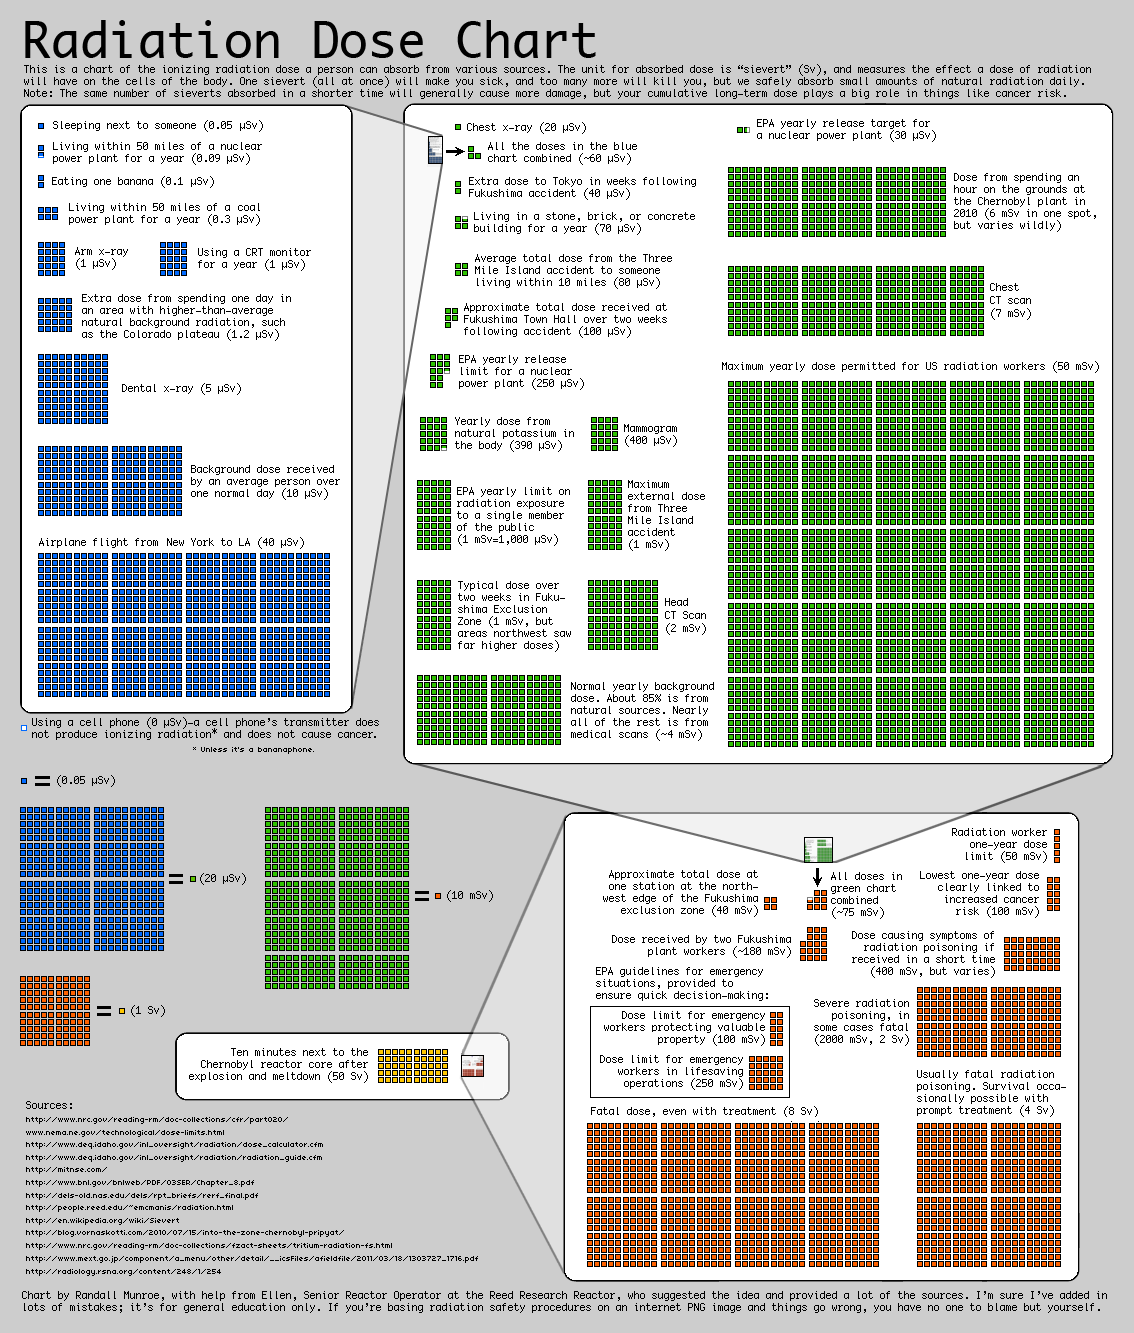
\includegraphics[width=\textwidth]{radioactivity-1/radiation-xkcd}
	\caption{A chart of ionizing radiation dose from various sources. Source: \url{https://xkcd.com/radiation/}}\label{rad1:doses}
\end{figure}

\subsection{Theory of counting statistics}

If you've ever worked in a not-too-busy retail environment, you’ve probably had the
experience of realizing (perhaps) that random and uniform are two quite different things.
You no doubt have sat waiting for customers, with nobody around for long stretches of
time, and then, as though they'd coordinated in advance, a half dozen people all show up
within a few minutes of each other. Each customer is indeed independent (no, they didn't
have a Twitter call to organize a flashmob!\footnote{Yes, popular interest in flash mobs peaked in 2011. Bear with us here.}) yet their arrival times clearly appear clustered. They are, in fact. But randomly. Uniform – one customer each minute – is quite dramatically different than a random procedure that yields one customer per minute on average. Retail customers (to a great extent), and elementary particles, act randomly, not uniformly.

Each atom in a radioactive sample has, per unit time, some probability of undergoing
radioactive decay. That probability is independent of all the other atoms in the sample.
Each atom decays, or not, based on its own probability and no other. The ensemble of
particle decay counts that one would measure in the sample (using a Geiger counter as we will
do, for example) is described by the something called the Poisson distribution, which
gives, in this instance, the probability of a integer number of events occurring in a fixed
interval of time, given an average rate. For large count rates, like we have here, the
Poisson distribution is indistinguishable from the normal distribution (that is, a simple
Gaussian function).

Specifically, for a process that produces an average $\bar{N}$ counts in a certain time duration (in the case of large $N$), the expected measurement of that count for that time duration is a
random draw from a normal distribution with mean $\bar{N}$ and a standard deviation of
$\sqrt{N}$.

	\begin{framed}
	\textbf{The Apparatus.}
	
	For this lab and the following one, you will be provided with a number of different radioactive materials packaged in small plastic disks. Note that each disk has the name of
	the isotope (e.g.\ $^{60}$Co), the type of radiation, and the half-life printed on one side of the
	sample. Half lives can range from fractions of a second to billions of years, depending on
	the isotope.
	
	The energetic particles produced in radioactive decay reactions can be detected by a
	device called a Geiger counter. This consists of a tube filled with inert gas with a wire
	running through it. A high voltage is applied between the wire and the tube. When a high-
	energy particle enters the tube, it can ionize the gas. The freed electrons produce a brief
	pulse of current at the output of the device. The pulses can then be counted.
	
	The counter itself is controlled using buttons on the front panel. \texttt{COUNT} begins the count
	and starts the timer, \texttt{STOP} pauses the count and timer, and \texttt{RESET} sets the count and
	timer to zero. Use the dial on the counter to change the display between the count and the
	elapsed time. When you first turn on the Geiger counter you need to set the voltage to
	$1000\:$V --- the TA will demonstrate how. \textbf{Caution:} Do not turn off the voltage during the
	experiment; use the \texttt{STOP} button to stop the count. \textbf{Do not touch the window on the
		bottom of the tube, as it breaks extremely easily.}
\end{framed}

\subsection{Procedure and analysis}

\begin{steps}
	\item To find the steps of a testing experiment, review Rubric C, found in Table~\ref{rubric:c}.
	
	\item\label{rad1:step:predict-random} A prediction is what the hypothesis says will happen in the event of a particular experimental procedure. Given the hypothesis stated in the goal, and the theory described above, if you collect a series of counts of radioactive decay, what does the hypothesis predict the standard deviation of those counts should be equal to? \textbf{Record this prediction in your lab notebook.}
	
	\item \textbf{Collecting data.} In order to find the standard deviation of a number of measurements, you will need to take those measurements. In the following steps, you will do 10 trials of measuring the count rate (counts per unit time) during periods of about 30 seconds, then take the standard deviation of those 10 trials. Since you will not be able to stop the counter after exactly 30 seconds, you will divide the displayed count by the displayed time to get a count rate (in units of ``counts per second''), and then multiply this by 30 to get the count-rate per 30 seconds.
	

	\begin{enumerate}
		\item \textbf{Take one of the $^{137}$Cs disks and place it} printed side down in the plastic shelf shaped to hold it, and place that shelf in the slot second from the top in the stand under the Geiger counter. Note that if you have the Geiger counter on, that it is measuring a large count rate.
		
		\item Use the controls \texttt{COUNT}, \texttt{STOP}, and \texttt{RESET} to \textbf{measure the number of counts in 10 approximately 30-second intervals.} Use the dial on the display to access both the counts and the elapsed time. The provided stopwatch may also help you organize your effort --- \textit{but use the time from the Geiger counter apparatus directly} for your calculations.
		
		\item \textbf{Record the counts and elapsed time in each interval in a spreadsheet} and calculate the count rate in counts per half-minute.
	\end{enumerate}

	\item \textbf{Analysis.} Note that the count rate is not identical in each trial, even though you accounted for the different measurement durations. Let's see how far away the standard deviation here is from the prediction in Step~\ref{rad1:step:predict-random}. Calculate the standard deviation of these measurements. How close is it? Answer this quantitatively by calculating the \textit{percent difference},
	\begin{equation}
	 \textrm{percent difference} = 200\% \times \frac{\abs{A - B}}{A+B} \,,
	\end{equation}
	where $A$ and $B$ are the two quantities that you are comparing. Without taking the time to find the uncertainty in the standard deviation, this is the best you can do to say how close it is.
	
%	\item Qualitatively, it might appear close or far away, but to test the hypothesis, you should take into account the uncertainty of the standard deviation. This is, effectively, the \textit{standard deviation of the standard deviation}. You would need to take, for example, 10 trials of these 10 trials and compute the standard deviation of that. Fortunately, you have other lab groups who are doing the same experiment. Share the standard deviation you found with the other lab groups, calculate the average and standard deviation of those standard deviations, and use Appendix~\ref{unc:sec:comparing} to compare your average standard deviation to the prediction that your hypothesis made.
	
	\item Use this quantitative comparison to determine if the prediction and the outcome agree or not.
	
	\item Based on that agreement, and taking into account the experimental conditions, make a judgment about the hypothesis. Is the radioactive decay happening randomly?
\end{steps}

\section{Observational experiment: types of radiation}

\textbf{Goal:} Observe the effects of shielding on different types of radiation and generate some ideas about the patterns you see.

\textbf{Rubrics to focus on:} F1, F2, G2. See Appendix~\ref{cha:rubrics} for details. \textit{Note that the C rubric rows from the previous experiment do not apply to an observational experiment.}

\textbf{Available equipment:} Stopwatch, SpecTech Geiger counter, computer with spreadsheet software, radioactive sources ($^{60}$Co, $^{137}$Cs, $^{90}$Sr), shielding of various thicknesses

\subsection{Background: types of radiation}

There are four basic types of radiation: alpha particles, which are the nuclei of helium
atoms consisting of two protons and two neutrons; beta particles, which are energetic
electrons; gamma rays, which are very energetic photons, \textit{i.e.}\ particles of light; and
finally neutrons. (The terms ``alpha,'' ``beta,'' and ``gamma'' were coined before anyone
knew much about the actual particles involved.) We’ll be working with gamma and beta
radiation in what follows. Next week's lab includes the use of a neutron
radiation source.

Different types of radiation of the same energy interact with matter in different ways.
Alpha is stopped by a piece of paper, beta is stopped by a book, while gamma rays are stopped by a shelf of books, or many inches of steel or lead.

\subsection{Procedure}

\begin{steps}
	\item We will begin by attempting to measure how much material it takes to stop the beta particles from $^{90}$Sr.
	Take a sample of $^{90}$Sr and put it under the Geiger counter in the second slot down from the top, printed side down, removing the $^{137}$Cs source you used previously if you still have it in place.
	
	\item Count the number of particles detected in 60 seconds from this source, and record this number.
	
	\item Qualitative observe the effect of different shields by placing them between the sample and the Geiger counter and recording the count rate (for example, in counts per minute) for each shield.
	You should try a few different shields with different thicknesses (measured in mg/cm$^2$).
	
	\item One way to quantity the penetrating ability of radiation is to find it's ``stopping length'', which is the thickness of shielding that reduces the detected count to half the unshielded amount. Find the stopping length of the radiation emitted by $^{90}$Sr and include uncertainties in your reported count rates.

	\item Now find the stopping length for $^{60}$Co. This time, \textbf{place the sample holder in the third slot from the top instead of the second}. If you need to use a thicker shield than the thickest one, you can use two of them and add the thicknesses together.
	
	\item How do the two stopping lengths compare, qualitatively, to each other. What does this tell you about the relative penetrating ability of beta and gamma radiation?
	
	\item As before, note your measured count rates, with uncertainties, in your lab report, as well as recording the stopping length.
	
	\item Now, finally, we will examine the radioactive properties of the $^{137}$Cs source.
	Place it in the sample holder as before, and record the unshielded count rate in a 60 second interval.
	The sample is noted as having both gamma and beta radiation.
	Use the shields to attempt to establish this experimentally, by comparison to the results you got for the $^{60}$Co and $^{90}$Sr samples. \textit{Note that this last step is not a standard part of an observational experiment, but rather an application experiment.}
	
\end{steps}

\subsection{Questions for discussion, to include in your lab report}

\begin{steps}

	\item How do the stopping lengths for beta particles compare to the stopping lengths for gamma rays? Can you come up with a physical explanation for the patterns you observe? Does this explanation extend to what you know about alpha particles?
	
\end{steps}

\section{Report checklist and grading}

Each item below is worth 10 points, and there is an additional 10 points for attendance and participation.

\begin{itemize}
	\item Prediction, data table from Steps 2--3.
	
	\item Analysis, percent difference, and conclusions from Steps 4--6.
	
	\item Procedure, relevant data (choose to use a data table or graph) for determining the stopping length of $^90$Sr (from Step 10).
	
	\item Your determination of the stopping length of $^90$Sr, with uncertainty estimate (Step 10).
	
	\item Procedure, data, analysis, and determination of $^60$Co stopping length (Steps 11, 13).
	
	\item Procedure and explanation with data for how you showed that $^137$Cs emits both beta and gamma radiation (Step 14).
	
	\item Question in Step 15.
\end{itemize}